\chapter{Proposed Methodology}
\label{chap:methodology}

\section{Overview of the Proposed Architecture}
\label{sec:method_overview}

To overcome the three core limitations of baseline LayoutLMv3 in Key Information Extraction (KIE)—namely isotropic 2D coordinate embeddings, the absence of explicit line/segment structural consensus, and the lack of intra-line boundary regularization—we propose a \textbf{Structure-Aware Multi-Modal LayoutLMv3 Architecture}.

Figure~\ref{fig:proposed_architecture} illustrates the complete end-to-end processing pipeline of our proposed model. The architecture augments the pre-trained LayoutLMv3 backbone~\cite{huang2022layoutlmv3} with three tightly coupled structural enhancements:
\begin{enumerate}
    \item \textbf{Hierarchical 2D Positional Encoding (HPE)} inside the input spatial embedding layer (\texttt{LayoutLMv3}\allowbreak\texttt{TextEmbeddings}), which decouples horizontal intra-line features $(x_0, x_1, w)$ from vertical inter-line features $(y_0, y_1, h)$ via asymmetric sub-embeddings and a non-linear hierarchical fusion block.
    \item \textbf{Token-Segment Interaction Module (Segment Consensus Module - SCM)} placed on top of the multi-modal Transformer encoder (\texttt{LayoutLMv3}\allowbreak\texttt{SegmentModel}), which aggregates subword token representations into line-segment embeddings, captures global inter-segment layout relationships via multi-head self-attention, and injects structural context back into each token via a \textbf{ReZero-style learnable scalar gate} $\alpha$ and a binary \textbf{segment-start indicator embedding}.
    \item \textbf{Intra-Line Boundary Regularization Loss ($\mathcal{L}_{\text{bound}}$)} in the sequence labeling head (\texttt{LayoutLMv3For}\allowbreak\texttt{TokenClassification}), which penalizes cosine representation divergence between consecutive tokens belonging to the same line segment and sharing the same base entity class.
\end{enumerate}

\begin{figure}[htbp]
\centering
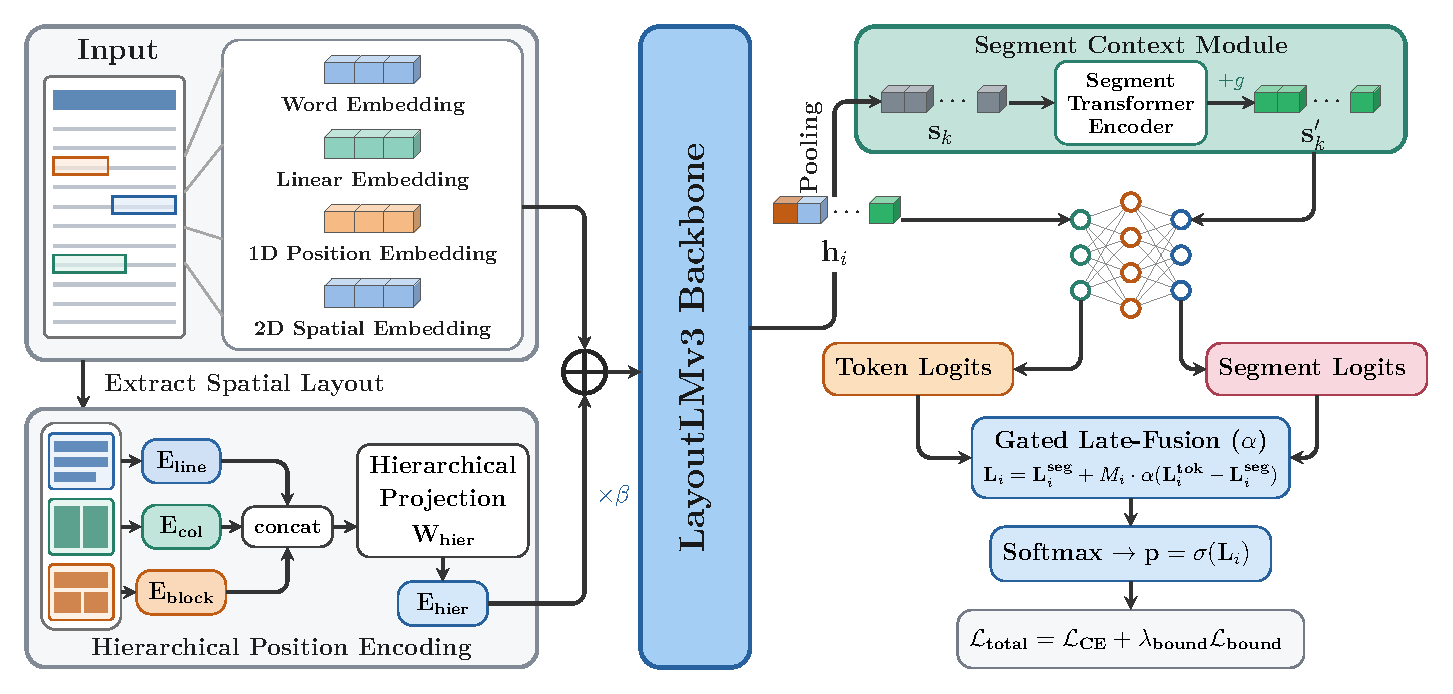
\includegraphics[width=\linewidth]{../figures/model_architecture_heads_style.pdf}
\caption{End-to-end architecture of our proposed Structure-Aware LayoutLMv3 framework for Key Information Extraction on Visually Rich Documents, featuring (1) Hierarchical Position Encoding (HPE), (2) Multimodal LayoutLMv3 Backbone, (3) Dual-Path Segment Context Module (SCM) with ReZero Gating, (4) Fine-Grained Token Identity Shortcut, and (5) Topological Masked Gated Late-Fusion supervised by Joint Cross-Entropy and Intra-Line Boundary Loss.}
\label{fig:proposed_architecture}
\end{figure}



\section{Component 1: Hierarchical 2D Positional Encoding (HPE)}
\label{sec:method_hpe}

\subsection{Limitation of Isotropic 2D Coordinate Embeddings}
In the standard LayoutLMv3 architecture~\cite{huang2022layoutlmv3}, given a normalized bounding box $\mathbf{b}_i = (x_0, y_0, x_1, y_1) \in [0, 1000]^4$ along with its width $w = \text{clip}(x_1 - x_0, 0, 1023)$ and height $h = \text{clip}(y_1 - y_0, 0, 1023)$, the baseline model allocates an identical embedding dimension $d_c = d / 6$ to all six spatial attributes:
\begin{equation}
    \mathbf{e}_{\text{base}}^{\text{pos2D}}(\mathbf{b}_i) = \left[ \mathbf{e}_x(x_0) \;\|\; \mathbf{e}_y(y_0) \;\|\; \mathbf{e}_x(x_1) \;\|\; \mathbf{e}_y(y_1) \;\|\; \mathbf{e}_w(w) \;\|\; \mathbf{e}_h(h) \right] \in \mathbb{R}^d,
    \label{eq:baseline_pos2d}
\end{equation}
where $\|$ denotes vector concatenation. For \texttt{layoutlmv3-base} ($d=768$), each attribute receives $d_c = 128$ dimensions; for \texttt{layoutlmv3-large} ($d=1024$), each attribute receives $d_c = 170$ dimensions. However, Equation~\ref{eq:baseline_pos2d} contains no cross-coordinate interaction layer and treats horizontal and vertical axes isotropically.

\subsection{Asymmetric Axis Decomposition and Hierarchical Fusion}
In document layouts, vertical coordinates $(y_0, y_1, h)$ govern macro-level reading progression across lines and hierarchical document sections, whereas horizontal coordinates $(x_0, x_1, w)$ encode micro-level intra-line word order and column alignment. To reflect this structural asymmetry, our \textbf{Hierarchical 2D Positional Encoding (HPE)} decouples the six spatial attributes into two distinct geometric groups with asymmetric subspace dimensions:
\begin{itemize}
    \item \textbf{Horizontal (Intra-Line) Subspace:} Each horizontal coordinate $x_0, x_1, w$ is embedded into dimension $d_x = d / 8$:
    \begin{equation}
        \mathbf{e}_{\text{horiz}}(\mathbf{b}_i) = \left[ \mathbf{e}_x^{\text{HPE}}(x_0) \;\|\; \mathbf{e}_x^{\text{HPE}}(x_1) \;\|\; \mathbf{e}_w^{\text{HPE}}(w) \right] \in \mathbb{R}^{3d_x}.
    \end{equation}
    \item \textbf{Vertical (Inter-Line) Subspace:} Each vertical coordinate $y_0, y_1, h$ is embedded into a higher-capacity subspace of dimension $d_y = \frac{d - 3d_x}{3} = \frac{5d}{24}$:
    \begin{equation}
        \mathbf{e}_{\text{vert}}(\mathbf{b}_i) = \left[ \mathbf{e}_y^{\text{HPE}}(y_0) \;\|\; \mathbf{e}_y^{\text{HPE}}(y_1) \;\|\; \mathbf{e}_h^{\text{HPE}}(h) \right] \in \mathbb{R}^{3d_y}.
    \end{equation}
\end{itemize}

Specifically, for \texttt{layoutlmv3-base} ($d=768$), we allocate $d_x = 96$ per horizontal coordinate ($3d_x = 288$) and $d_y = 160$ per vertical coordinate ($3d_y = 480$), summing exactly to $288 + 480 = 768$. For \texttt{layoutlmv3-large} ($d=1024$), we allocate $d_x = 128$ ($3d_x = 384$) and $d_y = 213$ (with residual padding integrated via linear projection to match $d = 1024$).

Furthermore, rather than passing the raw concatenation directly into the sum of token embeddings, HPE applies a non-linear \textbf{Hierarchical Fusion Projection} consisting of a learnable dense interaction matrix $\mathbf{W}_{\text{HPE}} \in \mathbb{R}^{(3d_x + 3d_y) \times d}$, bias $\mathbf{b}_{\text{HPE}} \in \mathbb{R}^d$, Layer Normalization, and a GELU activation function:
\begin{equation}
    \mathbf{e}_{\text{HPE}}^{\text{pos2D}}(\mathbf{b}_i) = \text{GELU}\!\left( \text{LN}\!\left( \mathbf{W}_{\text{HPE}} \left[ \mathbf{e}_{\text{horiz}}(\mathbf{b}_i) \;\|\; \mathbf{e}_{\text{vert}}(\mathbf{b}_i) \right] + \mathbf{b}_{\text{HPE}} \right) \right) \in \mathbb{R}^d.
    \label{eq:hpe_projection}
\end{equation}

This non-linear fusion allows the embedding layer to capture multiplicative aspect-ratio interactions (e.g., distinguishing wide full-page section headers from narrow tabular price cells) prior to entering the first Transformer layer.

\section{Component 2: Token-Segment Interaction Module (SCM)}
\label{sec:method_scm}

\subsection{Motivation and Multi-Granularity Formulation}
Let $\mathbf{H}_{\text{enc}} \in \mathbb{R}^{B \times (L + M + 1) \times d}$ denote the final hidden states produced by the LayoutLMv3 encoder for batch size $B$, text sequence length $L$, and visual patch length $M+1$. Extracting the text slice yields token-level representations $\mathbf{H} = (\mathbf{h}_1, \mathbf{h}_2, \dots, \mathbf{h}_L) \in \mathbb{R}^{B \times L \times d}$.

During data collation (\texttt{DataCollator}\allowbreak\texttt{ForKeyValueExtraction}), contiguous words sharing an identical line-level bounding box are grouped into $S$ distinct visual text segments indexed by $s_i \in \{0, 1, \dots, S-1\}$ (with padding tokens assigned $s_i = -1$). To enforce structural consensus across all tokens within a line segment and model layout dependencies across segments, we introduce the \textbf{Token-Segment Interaction Module} (implemented in \texttt{modeling\_}\allowbreak\texttt{layoutlmv3\_}\allowbreak\texttt{segment.py}).

\subsection{Step 1: Segment Representation Aggregation via Mean Pooling}
For each valid segment $k \in \{0, 1, \dots, S-1\}$ in a document sample, let $\mathcal{I}_k = \{ i \in \{1, \dots, L\} \mid s_i = k \}$ denote the set of token positions belonging to segment $k$. We construct the initial segment representation $\mathbf{u}_k \in \mathbb{R}^d$ via masked mean pooling over all constituent tokens:
\begin{equation}
    \mathbf{u}_k = \frac{1}{\max(|\mathcal{I}_k|, 1)} \sum_{i \in \mathcal{I}_k} \mathbf{h}_i, \quad k \in \{0, 1, \dots, S-1\}.
    \label{eq:segment_mean_pooling}
\end{equation}
Stacking all $S$ segments across the batch yields the segment tensor $\mathbf{U} = (\mathbf{u}_0, \dots, \mathbf{u}_{S-1}) \in \mathbb{R}^{B \times S \times d}$ alongside a boolean validity mask $\mathbf{M}_{\text{seg}} \in \{0, 1\}^{B \times S}$ indicating non-empty segments ($|\mathcal{I}_k| > 0$).

\subsection{Step 2: Inter-Segment Multi-Head Self-Attention}
To enable each text line to reason about its surrounding semantic context (e.g., linking a question segment on the left to an answer segment on the right, or linking a receipt header to a total row), we refine $\mathbf{U}$ through a dedicated Multi-Head Self-Attention block (\texttt{SegmentAttention}) with $H_{\text{seg}} = 8$ attention heads and head dimension $d_{\text{seg}} = d / H_{\text{seg}}$:
\begin{align}
    \tilde{\mathbf{U}} &= \text{MHSA}_{\text{seg}}\!\left(\mathbf{U}, \mathbf{U}, \mathbf{U}; \, \mathbf{M}_{\text{seg}}\right), \label{eq:segment_mhsa} \\
    \hat{\mathbf{U}} &= \text{LN}_{\text{seg}}\!\left( \mathbf{U} + \text{Dropout}\!\left(\mathbf{W}_{\text{seg}}^O \tilde{\mathbf{U}}\right) \right) \in \mathbb{R}^{B \times S \times d}. \label{eq:segment_ln}
\end{align}

\subsection{Step 3: ReZero-Gated Token-Segment Broadcast and Segment-Start Indicator}
After computing the refined segment representations $\hat{\mathbf{U}} = (\hat{\mathbf{u}}_0, \dots, \hat{\mathbf{u}}_{S-1})$, each token $i \in \{1, \dots, L\}$ with valid segment index $s_i \ge 0$ retrieves its corresponding refined line context $\hat{\mathbf{u}}_{s_i} \in \mathbb{R}^d$.

However, directly adding an randomly initialized attention module onto a pre-trained Transformer backbone during fine-tuning can destabilize early-epoch gradients—especially on compact datasets such as FUNSD (149 training pages). Furthermore, if all tokens inside segment $k$ receive the exact same broadcast vector $\hat{\mathbf{u}}_k$, the classifier may struggle to distinguish the opening token ($\texttt{B-}e_k$) from internal continuation tokens ($\texttt{I-}e_k$).

We solve both issues simultaneously through two mechanisms:
\begin{enumerate}
    \item \textbf{Binary Segment-Start Indicator Embedding ($\mathbf{e}_{\text{first}}$):}
    For each token $i$, we define a binary indicator $f_i \in \{0, 1\}$ that equals $1$ if and only if token $i$ is the very first token of its segment:
    \begin{equation}
        f_i = \mathds{1}\!\left[ s_i \ge 0 \;\wedge\; (i = 1 \;\vee\; s_i \neq s_{i-1}) \right].
        \label{eq:first_token_indicator}
    \end{equation}
    This indicator looks up a learnable embedding table $\mathbf{e}_{\text{first}}(f_i) \in \mathbb{R}^d$ (\texttt{is\_first\_}\allowbreak\texttt{token\_embedding}), explicitly signaling the structural boundary between $\texttt{B-}$ and $\texttt{I-}$ tags at the start of every visual segment.

    \item \textbf{ReZero-Style Learnable Scalar Gate ($\alpha$):}
    Inspired by ReZero~\cite{bachlechner2021rezero}, we introduce a learnable scalar parameter $\alpha \in \mathbb{R}$ initialized to $\alpha^{(0)} = 0.0$ (\texttt{segment\_gate} = \texttt{nn.Parameter(}\allowbreak\texttt{torch.zeros(1))}). The final structure-aware token representation $\mathbf{h}_i^{\text{final}} \in \mathbb{R}^d$ is computed as:
    \begin{equation}
        \mathbf{h}_i^{\text{final}} = \mathbf{h}_i + \alpha \cdot \mathds{1}[s_i \ge 0] \cdot \left( \hat{\mathbf{u}}_{s_i} + \mathbf{e}_{\text{first}}(f_i) \right).
        \label{eq:rezero_fusion}
    \end{equation}
\end{enumerate}

At initialization ($\alpha = 0$), Equation~\ref{eq:rezero_fusion} reduces exactly to the identity mapping $\mathbf{h}_i^{\text{final}} = \mathbf{h}_i$, preserving the exact pre-trained LayoutLMv3 feature manifold at step 0 and allowing the optimizer to gradually increase $|\alpha|$ as the segment attention weights warm up.

\section{Component 3: Intra-Line Boundary Regularization Loss}
\label{sec:method_boundary_loss}

\subsection{Standard Cross-Entropy Objective}
Given the refined token representations $\mathbf{H}^{\text{final}} = (\mathbf{h}_1^{\text{final}}, \dots, \mathbf{h}_L^{\text{final}}) \in \mathbb{R}^{B \times L \times d}$, the classification head applies dropout and a linear projection $\mathbf{W}_{\text{cls}} \in \mathbb{R}^{d \times |\mathcal{Y}|}$ to produce token logits $\mathbf{z}_i = \mathbf{W}_{\text{cls}}^\top \mathbf{h}_i^{\text{final}} + \mathbf{b}_{\text{cls}} \in \mathbb{R}^{|\mathcal{Y}|}$. Let $\mathcal{V}_{\text{valid}} = \{ i \in \{1, \dots, L\} \mid y_i \neq -100 \}$ denote the set of active (non-masked) token positions. The standard token classification Cross-Entropy loss is:
\begin{equation}
    \mathcal{L}_{\text{CE}} = -\frac{1}{|\mathcal{V}_{\text{valid}}|} \sum_{i \in \mathcal{V}_{\text{valid}}} \log \frac{\exp(z_{i, y_i})}{\sum_{c=1}^{|\mathcal{Y}|} \exp(z_{i, c})}.
    \label{eq:ce_loss}
\end{equation}

\subsection{Formulation of the Intra-Line Cosine Boundary Regularizer}
While $\mathcal{L}_{\text{CE}}$ supervises each token $i$ in isolation, it does not explicitly constrain adjacent tokens $(i, i+1)$ within the same visual text segment ($s_i = s_{i+1}$) to maintain smooth hidden state trajectories when they belong to the same semantic entity.

Let $\phi(y) \in \{0, 1, \dots, K\}$ denote a base-entity mapping function (\texttt{base\_labels}) that strips the $\texttt{B-}$/$\texttt{I-}$ prefix from IOB2 labels—mapping $\texttt{O} \mapsto 0$ and both $\texttt{B-}e_k, \texttt{I-}e_k \mapsto k$ via integer division $\lfloor (y + 1) / 2 \rfloor$. We define the set of valid intra-line homogeneous adjacent pairs $\mathcal{P}_{\text{intra}}$ as:
\begin{equation}
    \mathcal{P}_{\text{intra}} = \left\{ (i, i+1) \;\middle|\; i, i+1 \in \mathcal{V}_{\text{valid}}, \;\; s_i = s_{i+1} \ge 0, \;\; \phi(y_i) = \phi(y_{i+1}) \right\}.
    \label{eq:intra_line_pairs}
\end{equation}

For every adjacent pair $(i, i+1) \in \mathcal{P}_{\text{intra}}$, we measure the directional divergence between their structure-aware hidden representations $\mathbf{h}_i^{\text{final}}$ and $\mathbf{h}_{i+1}^{\text{final}}$ using cosine dissimilarity:
\begin{equation}
    d_{\cos}\!\left(\mathbf{h}_i^{\text{final}}, \mathbf{h}_{i+1}^{\text{final}}\right) = 1 - \frac{\langle \mathbf{h}_i^{\text{final}}, \, \mathbf{h}_{i+1}^{\text{final}} \rangle}{\|\mathbf{h}_i^{\text{final}}\|_2 \, \|\mathbf{h}_{i+1}^{\text{final}}\|_2 + \epsilon},
    \label{eq:cosine_dissimilarity}
\end{equation}
where $\epsilon = 10^{-8}$ ensures numerical stability. Averaging over all valid intra-line pairs yields the \textbf{Intra-Line Boundary Regularization Loss}:
\begin{equation}
    \mathcal{L}_{\text{bound}} =
    \begin{cases}
        \displaystyle \frac{1}{|\mathcal{P}_{\text{intra}}|} \sum_{(i, i+1) \in \mathcal{P}_{\text{intra}}} \left( 1 - \cos\!\left(\mathbf{h}_i^{\text{final}}, \mathbf{h}_{i+1}^{\text{final}}\right) \right), & \text{if } |\mathcal{P}_{\text{intra}}| > 0, \\[10pt]
        0, & \text{otherwise.}
    \end{cases}
    \label{eq:boundary_loss}
\end{equation}

\subsection{Joint Training Objective and Algorithmic Workflow}
Combining the primary sequence labeling loss (Equation~\ref{eq:ce_loss}) with our intra-line boundary regularizer (Equation~\ref{eq:boundary_loss}) produces the joint training objective:
\begin{equation}
    \mathcal{L}_{\text{total}} = \mathcal{L}_{\text{CE}} + \lambda_{\text{bound}} \, \mathcal{L}_{\text{bound}},
    \label{eq:total_loss}
\end{equation}
where $\lambda_{\text{bound}} \ge 0$ (\texttt{boundary\_loss\_}\allowbreak\texttt{weight}, set to $\lambda_{\text{bound}} = 0.2$ in our full model) controls the strength of intra-line smoothness regularization. Notably, $\mathcal{L}_{\text{bound}}$ is computed exclusively during training and introduces \textbf{zero computational overhead during inference}. Algorithm~\ref{alg:forward_training} summarizes the complete forward pass and joint loss computation of our proposed framework.

\begin{algorithm}[htbp]
\SetAlgoLined
\DontPrintSemicolon
\KwIn{Batch of tokenized documents $\mathcal{B} = \{(\mathbf{w}, \mathbf{B}_{\text{box}}, \mathbf{s}, \mathbf{I}, \mathbf{y})\}$; parameter $\lambda_{\text{bound}} = 0.2$.}
\KwOut{Token prediction logits $\mathbf{Z} \in \mathbb{R}^{B \times L \times |\mathcal{Y}|}$ and joint loss $\mathcal{L}_{\text{total}}$.}

\BlankLine
\textbf{Step 1: Hierarchical 2D Positional Encoding (HPE)}\;
\ForEach{token $i \in \{1, \dots, L\}$}{
    Embed horizontal coordinates $\mathbf{e}_{\text{horiz}}(\mathbf{b}_i)$ and vertical coordinates $\mathbf{e}_{\text{vert}}(\mathbf{b}_i)$\;
    Project hierarchically: $\mathbf{e}_{\text{HPE}}^{\text{pos2D}}(\mathbf{b}_i) \leftarrow \text{GELU}(\text{LN}(\mathbf{W}_{\text{HPE}}[\mathbf{e}_{\text{horiz}} \| \mathbf{e}_{\text{vert}}] + \mathbf{b}_{\text{HPE}}))$\;
    Form text input: $\mathbf{e}_i^{\text{text}} \leftarrow \text{LN}(\mathbf{e}^{\text{word}}(w_i) + \mathbf{e}^{\text{pos1D}}(i) + \mathbf{e}^{\text{type}}(0) + \mathbf{e}_{\text{HPE}}^{\text{pos2D}}(\mathbf{b}_i))$\;
}

\BlankLine
\textbf{Step 2: Multi-Modal Transformer Backbone Encoding}\;
Project visual patches $\mathbf{E}^{\text{image}} \in \mathbb{R}^{B \times (M+1) \times d}$ from document image $\mathbf{I}$\;
Encode multimodal sequence: $\mathbf{H}_{\text{enc}} \leftarrow \text{TransformerEncoder}([\mathbf{E}^{\text{text}} \| \mathbf{E}^{\text{image}}])$\;
Extract token states: $\mathbf{H} = (\mathbf{h}_1, \dots, \mathbf{h}_L) \leftarrow \mathbf{H}_{\text{enc}}[:, :L, :]$\;

\BlankLine
\textbf{Step 3: Token-Segment Interaction (SCM) with ReZero Gating}\;
\ForEach{segment index $k \in \{0, \dots, S-1\}$}{
    Mean pool segment tokens: $\mathbf{u}_k \leftarrow \frac{1}{\max(|\mathcal{I}_k|, 1)} \sum_{i \in \mathcal{I}_k} \mathbf{h}_i$\;
}
Refine segment context: $\hat{\mathbf{U}} \leftarrow \text{LN}_{\text{seg}}(\mathbf{U} + \text{Dropout}(\mathbf{W}_{\text{seg}}^O \text{MHSA}_{\text{seg}}(\mathbf{U})))$\;
\ForEach{token $i \in \{1, \dots, L\}$}{
    Indicator $f_i \leftarrow \mathds{1}[s_i \ge 0 \wedge (i = 1 \vee s_i \neq s_{i-1})]$\;
    Inject segment representation: $\mathbf{h}_i^{\text{final}} \leftarrow \mathbf{h}_i + \alpha \cdot \mathds{1}[s_i \ge 0] \cdot (\hat{\mathbf{u}}_{s_i} + \mathbf{e}_{\text{first}}(f_i))$\;
}

\BlankLine
\textbf{Step 4: Classification Logits \& Intra-Line Boundary Regularization}\;
Compute logits $\mathbf{Z} \leftarrow \text{Classifier}(\text{Dropout}(\mathbf{H}^{\text{final}})) \in \mathbb{R}^{B \times L \times |\mathcal{Y}|}$\;
Compute standard Cross-Entropy loss $\mathcal{L}_{\text{CE}}(\mathbf{Z}, \mathbf{y})$ over active tokens\;
Identify adjacent pairs: $\mathcal{P}_{\text{intra}} = \{(i, i+1) \mid s_i = s_{i+1} \ge 0, \, \phi(y_i) = \phi(y_{i+1})\}$\;
Compute cosine boundary loss: $\mathcal{L}_{\text{bound}} \leftarrow \frac{1}{|\mathcal{P}_{\text{intra}}|} \sum_{(i,i+1)} (1 - \cos(\mathbf{h}_i^{\text{final}}, \mathbf{h}_{i+1}^{\text{final}}))$\;
\Return{$\mathbf{Z}$ and $\mathcal{L}_{\text{total}} \leftarrow \mathcal{L}_{\text{CE}} + \lambda_{\text{bound}}\mathcal{L}_{\text{bound}}$}\;
\caption{Forward Propagation and Joint Training of Structure-Aware LayoutLMv3}
\label{alg:forward_training}
\end{algorithm}

